The aforementioned approaches to define linked data lifecycles, see Section~\ref{sect:related-work}, are based on performing some processes, 
recipes, methods or tasks using different tools to promote raw data as RDF triples. However, a formal definition of processes, 
methods and tasks is missing and, in most of the cases, they are based on the author’s expertise. The main consequence 
of this offhand mixing of approaches is the lack of a quantifiable method to measure the quality of the generated RDF. 
That is why we have selected and applied the lifecycle proposed in the MOLDEAS project~\cite{DBLP:journals/ijseke/AlvarezLSASL12}
that perfectly defines which the steps to produce, publish, consume and validate linked open data are. Figure~\ref{fig:summary-tasks} summarizes several 
tasks to be carried out in order to promote a controlled vocabulary to the Linked Data effort. The formal definition of processes, 
methods and tasks in this lifecycle enables separation of concerns and the sustainable management of linked data. In the e-Government 
area this issue must be addressed due to the implicit responsibility of the public administrations of delivering high-quality services and data.
\subsection{Least Common Multiple of Controlled Vocabularies}
As we have just introduced in the previous section, knowledge organizing systems are used for managing large collections of 
information objects and efficient information retrieval. Existing controlled vocabularies are currently available in several 
formats: PDF, MSExcel, CSV or XML. However promoting them to the Semantic Web is not a merely process of 
RDF/OWL conversions of data. Transformations need to fulfill some requirements. Firstly, a common RDF/OWL 
representation is required to ensure a) the semantic compatibility between different vocabularies,
b) the processing of vocabularies in a standard way and c) the sharing of vocabularies for third-parties adoption. 
SKOS, presented in the last W3C SKOS Core Recommendation, has been selected for these purposes. 
Secondly, although controlled vocabularies have some specific non-shared features, in practice a distinction 
between them is very hard to draw. We have identified a minimum set of common features for them. The data model 
should be expressive enough to preserve as much as possible the original semantics of primary sources for these 
common features. Thirdly, a generic method is needed to ensure quality of data conversions to correct SKOS instances. 
We have put in action the MOLDEAS lifecycle for thesauri conversions, by applying it to the PSCs field and taking into 
account their special features commented in a previous section making special emphasis in the next points:
\begin{enumerate}
 \item \textbf{URI Scheme generation.} Controlled structured vocabularies and conceptual resources are interpreted in SKOS as RDF 
 resources: in particular, instances of \texttt{skos:ConceptScheme} and \texttt{skos:Concept}. Thus they are referenced by 
 means of Uniform Resource Identifiers (URIs).  Although namespaces are out of the scope of our analysis, one 
 of the sub steps of the method is the generation of the \texttt{rdf:ID}s of \texttt{skos:Concept} and \texttt{skos:ConceptScheme} 
 from the original source's information. Usually controlled vocabularies provide unique identifiers for their terms or concepts. 
 The options are then the following ones:
 \begin{itemize}
  \item Generating new identifiers for the concepts of the vocabulary. This option introduces additional management. 
  A mapping between elements of the original source and identifiers should be maintained for updating purposes.
  \item Using the string of the preferred term. We would like to point out here that multilingual sources introduce a 
  factor of complexity that it is not present in monolingual systems. In European multilingual sources, this solution 
  implies selecting a preferred term in a given natural language, thus promoting one language over the others with a 
  possible non-desired political impact. In addition, a control procedure has to be established to ensure URI updating if the source term changes.
  \item Using the identifier code of an element. This solution avoids the problem of selecting one preferred language 
  to encode concept URIs. Moreover, codes are usually strings composed by a serial number 
  (legal URI characters) and it preserves the original semantics of a multilingual,
  where these codes identify unique terms or concepts and establish mappings between different languages. 
  This last option has been chosen keeping in mind the desired feature of having ``cool URIs'' to identify RDF resources.
 \end{itemize}

 \item \textbf{Hierarchy formalization.} From our point of view, one of the common aspects shared by 
 KOS is a hierarchy-based structure, at least by thesauri, taxonomies and by most of 
 classification schemes. Hierarchical relations establish links between conceptual resources, 
 showing that the semantics of a resource is, in some way, more general (``broader'') than other (``narrower''). 
 In SKOS, the properties \texttt{skos:broader} and \texttt{skos:narrower} are only used to assert hierarchical 
 statements between two conceptual resources. By the way, these properties are currently not defined 
 as transitive properties. Nevertheless, third-parties, if they consider valuable, can use an OWL reasoner 
 to infer the transitive closure of the hierarchy by means of both transitive super properties 
 \texttt{skos:broaderTransitive} and \texttt{skos:narrowerTransitive}.
 
 From a theoretical point of view, the transitive closure of hierarchical relations 
 of KOS is still an open issue. Transitive logical formalizations (e.g. using a Description Logics-based language, like SKOS/OWL) 
 of broader/narrower properties have some risks. Cycles can appear in the hierarchical-based structured 
 of controlled vocabularies. Even though, transitive closure of these properties can be useful for 
 search applications to expand original user-queries with terms hierarchically related. In our conversion-method, 
 we have followed the recommendation of the current SKOS specification.
 
 \item \textbf{Multilingual and lexical features.} Regarding European controlled vocabularies, 
 multilinguism is a critical issue, especially in the CPV vocabulary. 
 Thesaurus are accessible in $21$ ($23$) official languages of the European Union 
 (Bulgarian, Spanish, Czech, Danish, German, Estonian, Greek, English, French, Italian, Latvian, Lithuanian, 
 Hungarian, Dutch, Polish, Portuguese, Romanian, Slovak, Slovene, Finnish and Swedish) and others such as Croatian. 
 In SKOS conceptual resources are labeled with any number of lexical strings, in any given natural 
 language identified by the \texttt{xml:lang} attribute, following normative RDF/XML syntax. 
 One of these labels is selected as the \texttt{skos:prefLabel}for any given language, and the 
 others as values of \texttt{skos:altLabel}.
 
\end{enumerate}


\begin{figure}[ht]
\centering
	%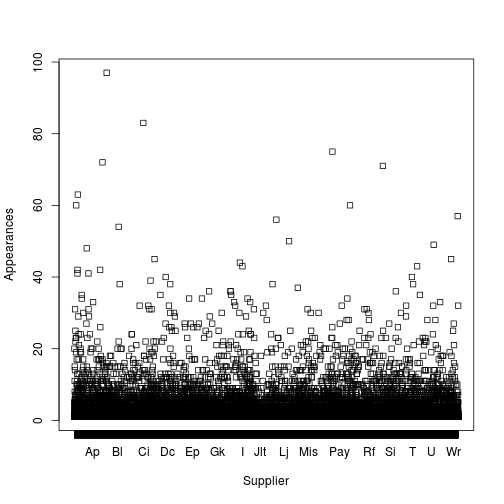
\includegraphics[width=\textwidth]{./imgs/corfu-stats}
 \caption{Summary of tasks of the MOLDEAS Linked Data lifecycle.}
 \label{fig:summary-tasks}
\end{figure}


% \begin{figure}[!h]
% \begin{center}
% \begin{lstlisting}[language=Python]  
% self.lemmatizer = nltk.WordNetLemmatizer()
% self.grammar = r"""
%   NBAR: {<NN.*|JJ>*<NN.*>}   
%   NP: {<NBAR>}
%       {<NBAR><IN><NBAR>} 
%     """
% self.chunker = nltk.RegexpParser(self.grammar)
% 
% def leaves(self, tree):
%   for subtree in tree.subtrees(filter = lambda t: t.node=='NP'):
%     yield subtree.leaves()
% \end{lstlisting}
% \caption{Regular expression-based chunker in Python NLTK and Filtering words by the category ``NP'' (noun phrase) .}
% \label{figure:step-4}
% \end{center}
% \end{figure}

